\chapter{Using objects}
	\label{ch:objects}

	This chapter explains:
	\begin{itemize}
		\item the use of instance variables and \keyword{Private};
		\item the form constructor;
		\item the use of library classes;
		\item the use of \keyword{New};
		\item using methods and properties;
		\item the \keyword{Random} class;
		\item the \keyword{TrackBar} and \keyword{Timer}.
	\end{itemize}


  \section{Introduction}
		In this chapter, we will deepen our understanding of objects. In particular, we will look at the use of different types of objects from the VB library of classes. Note that, though there are many hundreds of these, the principles of using them are similar.
		
		Here is an analogy: reading a book - whatever the book - involves opening it at the front, reading a page, then moving to the next page. We know what to do with a book. It is the same with objects. When you have used a few of them, you know what to look for when presented with a new one.
		
		In general, the objects we will make use of are termed controls or components. The terms are really interchangeable, but VB uses 'control' for items which can be manipulated on a form.

  \section{Instance variables}
		In order to tackle more advanced problems, we need to introduce a new place to declare variables. So far, we have used Dim to declare local variables within methods. But local variables alone are insufficient to tackle most problems.
	
		\begin{figure}[ht]
			\centering
			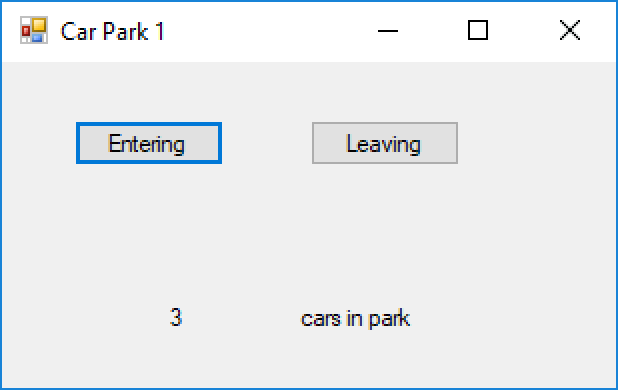
\includegraphics[width=8cm]{objects_carpark}
			\caption{Screenshot of Car park 1.}
			\label{fig:objects_carpark}
		\end{figure}
		Here we introduce a simple program (Car park 1) to assist in the running of a car park (or parking lot). It has two buttons: 'entering' and 'leaving'. The attendant clicks the appropriate button as a car enters or leaves. The program keeps a count of the number of cars in the park, and displays it in a label.
		
		Note that the count is changed by two methods, so it cannot be declared locally within only one of them. It is tempting to think that the variable can be declared within each method, but this would result in two separate variables.
		
		The screenshot is shown in \Vref{fig:objects_carpark}, and here is the code:
		\begin{lstlisting}
Public Class Form1
	Private carCount As Integer = 0
	Private Sub EnterButton_Click(
			sender As System.Object,	
			e As System.EventArgs) Handles EnterButton.Click
		carCount = carCount + 1
		CountLabel.Text = CStr(carCount)
	End Sub
	Private Sub LeaveButton_Click(
			sender As System.Object,
			e As System.EventArgs) Handles LeaveButton.Click
		carCount = carCount - 1
		CountLabel.Text = CStr(carCount)
	End Sub
End Class
		\end{lstlisting}
		There are a number of points to note:
		\begin{itemize}
			\item VB has automatically created a class named \keyword{Form1} for us. We have added two methods, \keyword{EnterButton\_Click} and \keyword{LeaveButton\_Click}, to the class. (We renamed the buttons to make the code more understandable.) We set the \keyword{Text} property of \keyword{Label1} to \keyword{0} at design-time.
			\item The variable \keyword{carCount} is declared \emph{outside} the methods, and \emph{inside} the class \keyword{Form1}. It can be used by any method in \keyword{Form1}.
			\item It has been declared as \keyword{Private}, meaning that any other classes we might have cannot use it. The variable is \emph{encapsulated} or sealed up inside \keyword{Form1}, i.e. it is for the use of the methods and properties of \keyword{Form1} only.
			\item \keyword{Dim} has not been used. We only use it for local variables.
			\item \keyword{carCount} is an example of an \emph{instance variable}. It belongs to an instance of a class, rather than to one method. Another term is 'class-level' variable.
			\item \keyword{carCount} is said to have \emph{module scope}. (A class is a type of module in VB.) The scope of an item is the area of the program in which it can be used. The other type of scope we have seen is local scope used with local variables.
			\item The word \keyword{Private} means that other classes (outside of our \keyword{Form1} class) cannot access the item. This is the preferred style for instance variables.
			\item The VB convention is not to capitalize the first letter of an instance variable.
		\end{itemize}
		Note that the programmer has free choice of names for instance variables. But what if a name coincides with a local variable name, as in:
		\begin{lstlisting}
Public Class Form1
	Private n As Integer = 8
	Private Sub MyMethod()
		Dim n As Integer
		n = 3	'which n?
	End Sub
End Class
		\end{lstlisting}
		Although both variables are accessible (in scope) within \keyword{MyMethod}, the rule is that the local variable is chosen. The instance variable (module-level) \keyword{n} remains set to \keyword{8}.

		\begin{stqb}
			\begin{STQ}
			\item	In the above \keyword{Form1} class, what are the consequences of deleting the \keyword{Dim} statement?
			\end{STQ}
		\end{stqb}
		Instance variables are essential, but you should not ignore locals. For example, if a variable is used inside one method only, and need not keep its value between method calls, make it local.


  \section{The form constructor}
	Let us re-visit the car park program. We used a variable \keyword{carCount} to count with, and we used a label to display the \keyword{carCount} value. We set the value of \keyword{carCount} to \keyword{0} within the program, and we set the \keyword{Text} property of \keyword{Label1} to 0 at design-time. In fact, these are not separate. Consider the possibility that five cars are left in the car park for an extended period. We have to alter the initial value of \keyword{carCount} as well as the initial value of the \keyword{Text} property of \keyword{Label1}. In reality, there is only one item holding the number of cars. This is \keyword{carCount}. Rather than separately setting the initial text value of \keyword{Label1} at design-time, it would be better to arrange that the value of \keyword{carCount} - whatever it is - is placed in the label as the program starts running.
		
		It is common for the initial values of controls to depend on variables and on other controls. We could attempt to set up this situation at design-time, but for several controls this is error-prone, and does not express the dependencies. It is better if we set up related initial values in code. Fortunately VB provides a special area of the program for such once-only initialization. Look at the second version: Car park 2.
		\begin{lstlisting}
Public Class Form1
	Private carCount As Integer = 0
	Public Sub New()
		' This call is required by the Windows Form Designer.
		InitializeComponent()
		' Add any initialization after the InitializeComponent() call.
		CountLabel.Text = CStr(carCount)
	End Sub
	Private Sub LeaveButton_Click(
			 sender As System.Object,
			 e As System.EventArgs) Handles LeaveButton.Click
		carCount = carCount - 1
		CountLabel.Text = CStr(carCount)
	End Sub
	Private Sub EnterButton_Click(
			 sender As System.Object,
			 e As System.EventArgs) Handles EnterButton.Click
		carCount = carCount + 1
		CountLabel.Text = CStr(carCount)
	End Sub
End Class
		\end{lstlisting}
		To create this code, we need to use the editor to open up an area of code that has not been explored before. Use your Car park 1 example, and view the code in the editor.
		\begin{itemize}
			\item In the two drop-down lists at the top of the editor, select \ui{Form1} and \ui{(Declarations)}.
			\item In the right drop-down list, select \ui{New}.
		\end{itemize}
		\begin{figure}[ht]
			\centering
			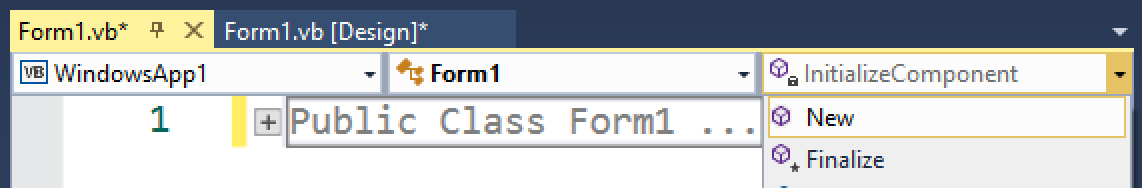
\includegraphics[width=10cm]{objects_form1_new}
			\caption{Showing the \ui{New} method.}
			\label{fig:objects_form1_new}
		\end{figure}

		\Vref{fig:objects_form1_new} shows the choice.
		
		You will see that another method has appeared in your code, headed:
		\begin{lstlisting}
Public Sub New()
		\end{lstlisting}
		When the VB system runs your program, it creates a new instance of \keyword{Form1}, and it calls its \keyword{New} method first. This method is known as a \emph{constructor} - it does some initial 'building' of the object. First, it creates your form and its controls by calling the \keyword{InitializeComponent} method. After the controls are created, you can write code to modify their initial values.
		
		You can imagine that the \keyword{New} method is always there, but does not need modifying in some introductory programs. For this reason, it is not shown. However, in this 
chapter, we will edit it.
		
		Look at the above code. You will see that it is composed of three methods: \keyword{New}, \keyword{LeaveButton\_Click} and \keyword{EnterButton\_Click}. In fact, the order of the methods does not matter. It is a convention in object-oriented programming to show the constructor method at the top, and we follow the convention here. However, the VB IDE places the methods in order of addition, so if you add \keyword{New} after creating the event code, \keyword{New} goes at the bottom. If you want to follow the convention, select \ui{View Code} then add \keyword{New} first, or cut and paste it to the appropriate position. Programs run fine even if the \keyword{New} method is not at the top of the code.

		In this improved version of the program, we have no need to set the \keyword{Text} of the label at design-time - instead, we insert code to do it towards the end of \keyword{New}, and the value is guaranteed to be the same as \keyword{carCount}. The comment:
		\begin{lstlisting}
'Add any initialization...
		\end{lstlisting}
		in the code shows you where it is safe to put your initialization. Do not put it anywhere else.
		
		\begin{stqb}
			\begin{STQ}
				\item	What is wrong with:
					\begin{lstlisting}
Public Sub New()
	... etc
	Label1.Text = "38"
	InitializeComponent()
End Sub
					\end{lstlisting}
			\end{STQ}
		\end{stqb}
		In the above example, we modified the \keyword{New} constructor, but did not call it ourselves. Later in this chapter, we will create new objects by explicitly calling the constructor of their class.


  \section{The \keyword{TrackBar} class}
		Here is another example of component initialization. The track bar is a GUI control from the toolbox. Open up \ui{All Windows Forms} to make it visible. It is similar in nature to the scroll bar at the side of a word-processor window, but the track bar can be placed anywhere on a form. The user can drag the 'thumb' to the required position, and the minimum and maximum values can be set via properties - at design-time and run-time.
		
		The track bar is not used for precise settings such as entering your age, where the range might be large, i.e. 10 to 100. It is used for more informal settings, such as setting the volume of a loudspeaker.
		
		Here we look at a program (Oval Shape) which allows the user to modify the width and the height of an ellipse. The current dimensions are displayed on the form in labels. \Vref{fig:objects_oval} shows a screenshot, and the code is shown overleaf:
		\begin{figure}[ht]
			\centering
			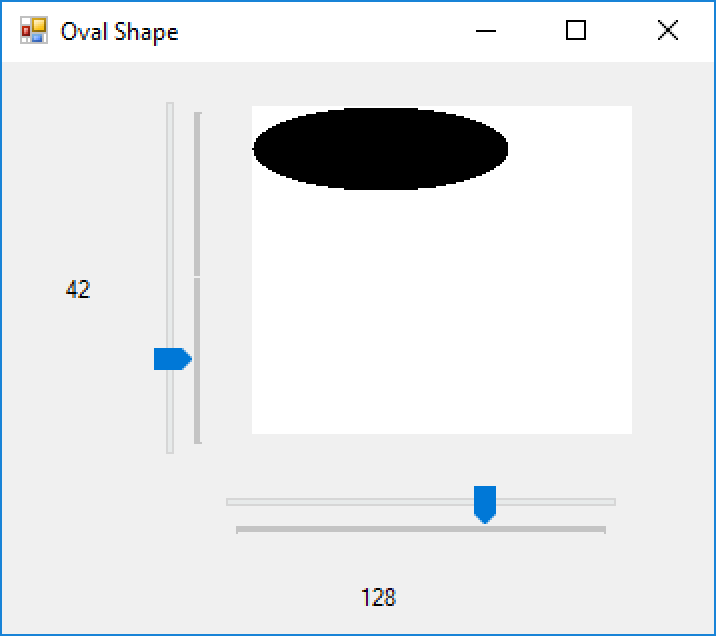
\includegraphics[width=10cm]{objects_oval}
			\caption{Screenshot of Oval Shape.}
			\label{fig:objects_oval}
		\end{figure}

		\begin{lstlisting}
Public Class Form1
	Private paper As Graphics
	Public Sub New()
		' This call is required by the Windows Form Designer.
		InitializeComponent()
		' Add any initialization after the InitializeComponent() call.
		paper = PictureBox1.CreateGraphics()
		VertTrackBar.Minimum = 0
		VertTrackBar.Maximum = PictureBox1.Height
		VertLabel.Text = CStr(VertTrackBar.Value)
		HorizTrackBar.Minimum = 0
		HorizTrackBar.Maximum = PictureBox1.Width
		HorizLabel.Text = CStr(HorizTrackBar.Value)
	End Sub
	Private Sub VertTrackBar_Scroll(
			 sender As System.Object,
			 e As System.EventArgs) Handles VertTrackBar.Scroll
		Dim myBrush As SolidBrush = New SolidBrush(Color.Black)
		VertLabel.Text = CStr(VertTrackBar.Value)
		paper.Clear(Color.White)
		paper.FillEllipse(myBrush, 0, 0, HorizTrackBar.Value,
			VertTrackBar.Value)
	End Sub
	Private Sub HorizTrackBar_Scroll(
			 sender As System.Object,
			 e As System.EventArgs) Handles HorizTrackBar.Scroll
		Dim myBrush As SolidBrush = New SolidBrush(Color.Black)
		HorizLabel.Text = CStr(HorizTrackBar.Value)
		paper.Clear(Color.White)
		paper.FillEllipse(myBrush, 0, 0, HorizTrackBar.Value,
			VertTrackBar.Value)
	End Sub
End Class
		\end{lstlisting}
		Here are some points on design-time initialization:
		\begin{itemize}
			\item The track bars have been renamed as \keyword{HorizTrackBar} and \keyword{VertTrackBar}.
			\item A track bar can be positioned vertically, by setting its \ui{Orientation} property to \ui{Vertical}.
			\item The labels have been renamed as \keyword{HorizLabel} and \keyword{VertLabel}.
			\item We set the picture box to a size of \keyword{100}, \keyword{100}.
		\end{itemize}
		At run-time, we used the constructor to initialize some components:
		\begin{itemize}
			\item We set the \keyword{Minimum} property of the track bars to \keyword{0}, and the \keyword{Maximum} properties to the height and width of the picture box.
			\item The initial value of the \keyword{Text} property of \keyword{HorizLabel} - which displays the current track bar value - is set to \keyword{HorizTrackBar.Value}. \keyword{VertTrackbar} is initialized in a similar way.
		\end{itemize}
		Note that:
		\begin{itemize}
			\item The track bar's event method (\keyword{Scroll}) is called when we move it to a new position.
			\item The track bar's \keyword{Value} property gives us the current setting. We use this to control the size of an imaginary rectangle enclosing the oval.
			\item The drawing area is used by two methods, so it must be declared as an instance variable at class-level, above the methods.
		\end{itemize}
		This program illustrates the benefits of initializing components in the form's constructor.
		
		\begin{stqb}
			\begin{STQ}
				\item	In the track bar example, what are the consequences of altering the size of the track bar at design-time?
			\end{STQ}
		\end{stqb}

	\section{\keyword{Imports} and namespaces}
		VB comes with a huge library (or collection) of classes which we can use. A very important aspect of VB programming is to make use of these, rather than write our own code. This is termed 'software reuse'.

		Because there are thousands of classes, they are subdivided into groups known as \emph{namespaces}. To use a class, we must ensure that it has been imported into our program. However, there are two possibilities, because some of the most frequently used namespaces are automatically imported into any Windows application. These namespaces are:
		\begin{lstlisting}
System
System.Data
System.Drawing
System.Windows.Forms
System.XML
		\end{lstlisting}
		There is a decision:
		\begin{itemize}
			\item if the class we require is in one of the above namespaces, we can use it with no further action;
			\item if the class we require is not in one of the above namespaces, we should put an \keyword{Imports} at the top of our program.
		\end{itemize}
		Here is an example. When we use files in \Cref{ch:files}, we will see the use of \keyword{StreamReader}, as in:
		\begin{lstlisting}
Dim myStream As StreamReader
		\end{lstlisting}
		The \keyword{StreamReader} class is in the \keyword{System.IO} namespace, so we must place the line:
		\begin{lstlisting}
Imports System.IO
		\end{lstlisting}
		at the very top of our code.
		There are two points to note:
		\begin{itemize}
			\item The importing does not work in a hierarchical way. Importing the \keyword{System} namespace does not automatically import every namespace which starts with \keyword{System}. Every namespace must be imported explicitly.
			\item The use of \keyword{Imports} merely provides us with a shorthand. For example, we could use the \keyword{StreamReader} class without importing, but we would have to put:
				\begin{lstlisting}
Dim myStream As System.IO.StreamReader
				\end{lstlisting}
		\end{itemize}
		To summarize, the vast library of VB classes is organized into namespaces, which can be imported into any program. When you have imported your class, you need to know how to create a new instance, and how to use its properties and methods. We shall look at these areas in a range of classes.


  \section{Members, methods and properties}
		The members of a class are its properties and its methods. Properties contain values which represent the current state of an instance of a class (such as the text contained in a label), whereas methods cause an instance to do a task - such as drawing a circle.
		
		Properties can be used in a similar manner to variables: we can place a new value in them, and access their current value. As an example, here is how the Width and Height properties of a label might be manipulated:
		\begin{lstlisting}
'set a new value in a property:
Label1.Height = 30
Label1.Height = CStr(TextBox1.Text)
'get current value of property:
Dim a As Integer
a = Label1.Height
a = label1.Height * Label1.Width
		\end{lstlisting}
		In VB terminology, we can \emph{set} a property to a new value and \emph{get} the current value of a property. Each one also has a type. For example, the Width property of the label holds an integer, whereas the \keyword{Text} property holds a string. The names and types of properties are available from the Help system.


		\begin{stqb}*
			\begin{STQ}
				\item	Imagine a CD player; list some methods and properties that it has. Which of these are members?
				\item In geometrical terms, what do the following statements accomplish?
					\begin{lstlisting}
a = Label1.Width * Label1.Height
Label1.Height = Label1.Width
					\end{lstlisting}
			\end{STQ}
		\end{stqb}
  

	\section{The \keyword{Random} class}
	Here we will look at a class (\keyword{Random}) which needs explicit declaration and initialization. \keyword{Random} numbers are very useful in simulations and in games; for example we can give the game-player a different initial situation every time. Instances of the \keyword{Random} class provide us with a 'stream' of random numbers, which we can obtain one-at-a-time via the \keyword{Next} method. Here is a program (Guesser) which attempts to guess your age (in a rather inefficient way) by displaying a sequence of random numbers. When you click on 'correct', the program displays the number of guesses it took. The screenshot is in \Vref{fig:objects_guesser}, and here is the code:
		\begin{figure}[ht]
			\centering
			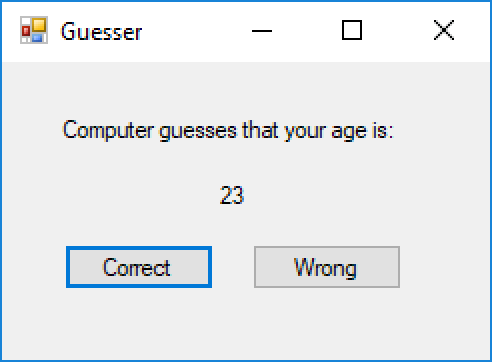
\includegraphics[width=7cm]{objects_guesser}
			\caption{Screenshot of Guesser.}
			\label{fig:objects_guesser}
		\end{figure}

		\begin{lstlisting}
Public Class Form1
	Private ageGuesser As Random = New Random()
	Private tries As Integer = 0
	Public Sub New()
		' This call is required by the Windows Form Designer.
		InitializeComponent()
		' Add any initialization after the InitializeComponent() call.
		GuessLabel.Text = CStr(ageGuesser.Next(5, 110))
	End Sub
	Private Sub CorrectButton_Click(
			 sender As System.Object,
			 e As System.EventArgs) Handles CorrectButton.Click
		tries = tries + 1
		MessageBox.Show("Number of tries was: " & CStr(tries))
		tries = 0
		GuessLabel.Text = CStr(ageGuesser.Next(5, 110))
	End Sub
	Private Sub WrongButton_Click(
			 sender As System.Object,
			 e As System.EventArgs)	Handles WrongButton.Click
		GuessLabel.Text = CStr(ageGuesser.Next(5, 110))
		tries = tries + 1
	End Sub
End Class
		\end{lstlisting}
		To use a new class, we use the Help system to find its namespace, and we put the appropriate \keyword{Imports} at the top of our program. The \keyword{Random} class turns out to be in the \keyword{System} namespace, which is imported automatically. No imports are needed in this program.
		
		We must then declare and initialize an instance of our class. This can be done in two ways. First we can use one statement, as in
		\begin{lstlisting}
Private ageGuesser As Random = New Random()
		\end{lstlisting}
		Note that:
		\begin{itemize}
			\item We chose the name \keyword{ageGuesser} for our instance.
			\item The statement calls the constructor of the \keyword{Random} class, which always has the same name as the class itself. The constructor is basically a method.
			\item The word \keyword{New} precedes the use of the constructor. \keyword{New} creates a new instance of a class in RAM.
			\item Constructors may be overloaded, so you need to choose the most convenient constructor. \keyword{Random} has two constructors, and the one with no parameters is suitable here.
			\item You can consider the statement to be in two parts:
				\begin{lstlisting}
Private ageGuesser As Random...
and
... = New Random()
				\end{lstlisting}
				The first part declares \keyword{ageGuesser} as a variable of class \keyword{Random}, but it does not yet have a concrete instance (containing methods and property values) associated with it. The second part calls the constructor of the \keyword{Random} class to complete the task of declaring and initialization.
		\end{itemize}

		The second way to declare and initialize instances is with declaration and initialization in different areas of the program, as in
		\begin{lstlisting}
Public Class Form1
	Private ageGuesser As Random
...
	ageGuesser = New Random()
		\end{lstlisting}
		Whichever approach we choose, there are a number of points:
		\begin{itemize}
			\item The declaration establishes the class of the instance. Here it is an instance of \keyword{Random}.
			\item The declaration establishes the scope of the object. \keyword{AgeGuesser} has module scope - it can be used by any method of the \keyword{Form1} class, rather than being local to a method.
			\item \keyword{ageGuesser} is private. It cannot be used by other classes outside our \keyword{Form1} class. Normally we make all such variables private.
			\item The initialization must be within the form's constructor or within another method.
			\item When it is possible to use the single-statement form of declaration and initialization, do so.
		\end{itemize}
		Why would we need to separate declaration and initialization? The situation often exists where we need an instance variable (as opposed to a local variable). It must be declared outside of the methods. But sometimes we cannot initialize the object until the program starts running - maybe the user enters a data value to be passed as a parameter to the constructor.
		
		In this case, we would put the initialization code inside a method (or perhaps the constructor). We cannot put the declaration within the method, as this would declare the item as local to the method.
		
		Let us return to the \keyword{Random} program. So far, we have created an instance of the \keyword{Random} class, named \keyword{ageGuesser}. We have yet to create any actual random numbers.
		
		Once an object has been created with \keyword{New}, we can use its properties and methods. The documentation tells us that there are several methods which provide us with a random number, and we chose to use the method which lets us specify the range of the numbers. The method is named \keyword{Next} (in the sense of fetching the next random number from a sequence of numbers). In our program, we put:
		\begin{lstlisting}
GuessLabel.Text = CStr(ageGuesser.Next(5, 110))
We could have coded it less concisely as:
Dim guess As Integer
guess = ageGuesser.Next(5, 110)
GuessLabel.Text = CStr(guess)
		\end{lstlisting}
		The range of random numbers was chosen to be 5 to 109 inclusive. The second parameter of \keyword{Next} is one greater than the largest number we require.

		To summarize, we declare an instance of the appropriate class (\keyword{Random} here), and use \keyword{New} to create and initialize it. These two stages can be combined, or separated; it depends on the particular program you are working on. Then we use properties and methods of the instance. The documentation provides us with details of their names and the types of data/parameters they require.

		\begin{stqb}
			\begin{STQ}
				\item	I went to my car sales showroom and, after browsing through the brochure, I ordered a specially built 5-litre Netster in blue. When it arrived, I drove it away. Does the Car class have a constructor? Does the constructor have any parameters? Which is the instance - the photo of the car or the real car?
			\end{STQ}
		\end{stqb}


	\section{The \keyword{Timer} class}
		So far, the classes we have used have fallen into two groups:
		\begin{itemize}
			\item Those from the toolbox, such as the button. They have a design-time representation on the form (e.g. they can be re-sized). They bring event-handling code templates with them, and code to call their constructors will automatically 
be placed in your code. Their initial properties can be set at design-time.
			\item Those from the libraries, without a visual representation - such as \keyword{Random}. 
		\end{itemize}
		They do not appear at design-time, and we have to explicitly code up a call to its constructor. Properties can only be set at run-time.
		
		The timer is slightly different: it is in the toolbox (open \ui{All Windows Forms}), but when it is dropped on to a form, the IDE opens up a new \ui{Component Tray} window below the design form, and puts a timer icon (a clock) on it. We can set properties at design-time, and double-clicking on the icon takes us to the timer's event-handling code. When we run the program, the timer does not appear on the form.
		
		Here are the main timer facilities:
		\begin{itemize}
			\item The timer creates ticks at regular intervals. Each tick is an event which calls the \keyword{Tick} method.
			\item The \keyword{Interval} property can be set to an integer value, representing the time between ticks in milliseconds.
			\item We can start and stop a timer with \keyword{Start} and \keyword{Stop} methods.
			\item We can put any number of timers in a program, each with a different interval.
		\end{itemize}
		Here is a program (Raindrops) which simulates a sheet of paper left out in the rain. It shows random-sized drops falling, at random intervals. The random intervals can be changed via a track bar. \Vref{fig:objects_raindrops} shows a screenshot, and here is the code:
		\begin{figure}[ht]
			\centering
			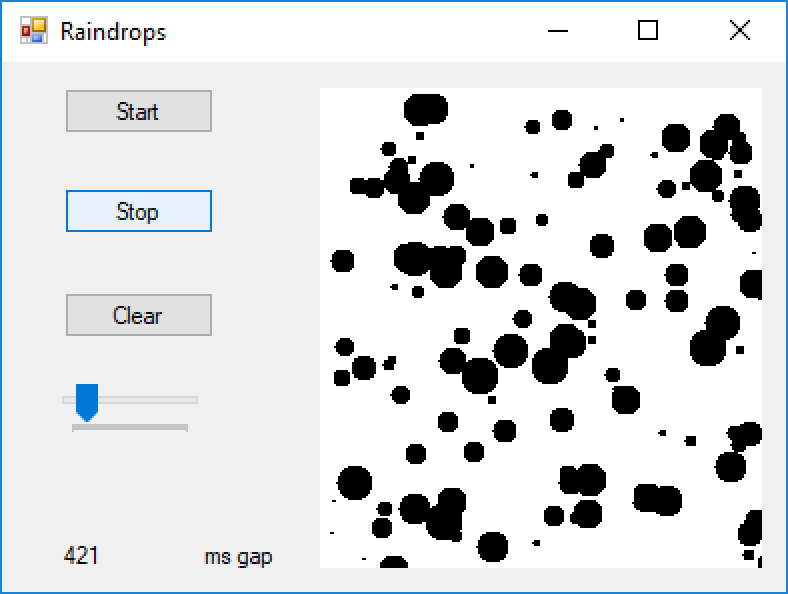
\includegraphics[width=7cm]{objects_raindrops}
			\caption{Screenshot of Raindrops.}
			\label{fig:objects_raindrops}
		\end{figure}

		\begin{lstlisting}
Public Class Form1
	Private randomNumber As Random = New Random()
	Private paper As Graphics
	Public Sub New()
		'This call is required by the Windows Form Designer.
		InitializeComponent()
		'Add any initialization after the InitializeComponent() call
		paper = PictureBox1.CreateGraphics()
		GapLabel.Text = CStr(TrackBar1.Value)
	End Sub
	Private Sub StartButton_Click(
			 sender As System.Object,
			 e As System.EventArgs)	Handles StartButton.Click
		Timer1.Start()
	End Sub
	Private Sub StopButton_Click(
			 sender As System.Object,
			 e As System.EventArgs) Handles StopButton.Click
		Timer1.Stop()
	End Sub
	Private Sub ClearButton_Click(
			sender As System.Object,
			 e As System.EventArgs)	Handles ClearButton.Click
		paper.Clear(Color.White)
	End Sub
	Private Sub Timer1_Tick( sender As System.Object,
			 e As System.EventArgs)	Handles Timer1.Tick
		Dim x, y, size As Integer
		Dim myBrush As Brush = New SolidBrush(Color.Black)
		x = randomNumber.Next(0, PictureBox1.Width)
		y = randomNumber.Next(0, PictureBox1.Height)
		size = randomNumber.Next(1, 20)
		paper.FillEllipse(myBrush, x, y, size, size)
		'set new interval for timer
		Timer1.Stop()
		Timer1.Interval =
			randomNumber.Next(1, TrackBar1.Value)
		Timer1.Start()
	End Sub
	Private Sub TrackBar1_Scroll(
				 sender As System.Object,
				 e As System.EventArgs)	Handles TrackBar1.Scroll
		Dim timeGap As Integer = TrackBar1.Value
		GapLabel.Text = CStr(timeGap)
	End Sub
End Class
		\end{lstlisting}
		The program works by drawing a randomly sized filled circle at a random position at every tick. We also reset the timer interval to a random value controlled by the track bar. (This necessitates stopping and starting the timer.) Each time the track bar is moved, we display its current value in a label. The \keyword{Minimum} and \keyword{Maximum} track bar values were chosen by experimentation, and are 200 and 2000, set at design-time. We also made use of the \keyword{Clear} method of the picture box, which sets all the box to a specified colour.

		\begin{stqb}
			\begin{STQ}
				\item	We have a timer with an interval set to 1000, i.e. one second. Explain how we can get a display of minutes on the form.
			\end{STQ}
		\end{stqb}


	\section{Programming principles}
		For many years it has been the dream of programmers to be able to build programs in the same way that hi-fi systems are built - i.e. from 'off-the-shelf' components, such as speakers, amplifiers, volume controls, etc. The rise in object-oriented programming has made this more possible, and it is used to some extent in the C++ and Java languages. However, the largest example of software reuse is that shown by earlier versions of VB, and this is likely to continue as VB becomes more widespread. Thousands of prepackaged VB controls are available, to do such tasks as speech recognition and Internet access. In VB, it is possible to write new controls for use by other programmers.
		
		Such controls are simple to incorporate: they are added to a project by a menu action. From then on, they appear on the toolbox like any other control, and provide event-handling method headers and properties that can be set at design-time. In practical terms, it is well worth searching for an existing control which meets your requirements, rather than reinventing the wheel by coding from scratch.


	\section{Programming pitfalls}
	If an instance is declared but its initialization with \keyword{New} is omitted, a run-time error is produced, of type \keyword{System.NullReferenceException}. Run-time errors (i.e. bugs) are more problematic than compile-time errors; they are harder to find, and they are more serious, because the program's execution is halted. We guarantee that you will meet this error!


	\section{Grammar spot}
		\begin{itemize}
			\item Instance variables are declared outside methods, using \keyword{Private}, as in:
				\begin{lstlisting}
Private yourVariable As Integer
Private myVariable As Random = New Random()
				\end{lstlisting}
			\item Instance variables can be initialized at declaration time, or inside a constructor or method.
			\item Properties can be manipulated in a similar manner to variables: we can get and set their values.
		\end{itemize}


	\section{New language elements}
		\begin{itemize}
			\item Private instance (class-level) variables.
			\item Using \keyword{New} for initialization.
			\item \keyword{Imports} for namespaces.
			\item The \keyword{TrackBar}, \keyword{Random} and \keyword{Timer} classes.
		\end{itemize}


	\section{New IDE facilities}
		The component tray, for controls that do not have a visual representation on a form.


	\section{Summary}
		The VB system has a vast number of classes which you can (and ought to) use. As well as the control classes which are in the toolbox, there are classes which can be incorporated into your programs by using \keyword{Imports} and the appropriate constructor.

	\section{Exercises}
		\begin{EXE}
			\item	Place a track bar on a form, together with two text boxes and a button. When the button is clicked, the track bar's \keyword{Minimum} and \keyword{Maximum} properties should be set from numbers entered in the text boxes. When the track bar is scrolled, display its \keyword{Minimum} and \keyword{Maximum} properties in message boxes.
			\item Write a program which initially displays the number \keyword{1} in a label. Clicking a button should increment the value. Make use of a private variable initialized to \keyword{1}, and set up the label in the constructor.
			\item Write a program which produces a random number between 200 and 400 each time a button is clicked. The program should display this number, and the sum and average of all the numbers so far. As you click again and again, the average should converge on 300. If it doesn't, we would suspect the random number generator - just as we would be suspicious of a coin that came out heads 100 times in a row!
			\item 
				\begin{enumerate}[label=(\alph*)]
					\item	Write a program which converts degrees Celsius to degrees Fahrenheit. The Celsius value should be entered in a text box. Clicking a button should cause the Fahrenheit value to be displayed in a label. The conversion formula is:
						\begin{equation*}
							f = c * 9 / 5 + 32
						\end{equation*}
					\item Modify the program so that the Celsius value is entered via a track bar, with its minimum set to 0, and its maximum set to 100.
					\item Represent both the temperatures as long thin rectangles in a picture box.
				\end{enumerate}
			\item Write a program which calculates the volume of a swimming pool, and which also displays its cross-section in a picture box. The width of the pool is fixed at 5 metres and the length is fixed at 20 metres. The program should have two track bars - one to adjust the depth of the deep end, and one to adjust the depth of the shallow end. The minimum depth of each end is 1 metre. Choose suitable values for the maximum and minimum track bar values at design time. The volume formula is:
				\begin{equation*}
					v = \text{averageDepth} * \text{width} * \text{length}
				\end{equation*}
				\begin{figure}[ht]
					\centering
					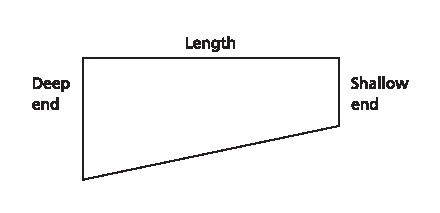
\includegraphics[width=8.5cm]{objects_swimming_pool}
					\caption{Swimming pool cross-section.}
					\label{fig:objects_swimming_pool}
				\end{figure}

				\Vref{fig:objects_swimming_pool} shows the cross-section.
			\item Write a program which displays changing minutes and seconds, representing them by two long rectangles: make the maximum width of the rectangles equal to 600 pixels to simplify the arithmetic (10 pixels for each minute and each second). Redraw the two rectangles every second. \Vref{fig:objects_time_display} shows a representation of 30 minutes and 15 seconds.
				\begin{figure}[ht]
					\centering
					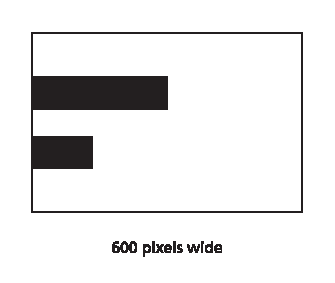
\includegraphics[width=7cm]{objects_time_display}
					\caption{Time display for 30 mins, 15 secs.}
					\label{fig:objects_time_display}
				\end{figure}

				
				The program should count up in seconds with a timer, and display the total seconds, and the time in minutes and seconds. Recall that, given a total number of seconds, we can use the Mod operator to break it down into whole hours and seconds remaining. In order to speed up testing the program, you should reduce the timer interval from 1000 milliseconds to, say, 200.
			\item This question guides you through the writing of a geometry game:
				\begin{enumerate}[label=(\alph*)]
					\item	Write a program with two track bars which control the horizontal and vertical position of a circle of 200 pixels diameter.
					\item Add a third track bar to control the diameter of the circle.
					\item What follows is a game based on the mathematical fact that a circle can be drawn through any three points. The program should display 3 points (each is a small filled circle) when a 'Next Game' button is clicked. Good initial positions are (100,100), (200,200), (200,100) but you can add a small random number to them for variety. The player has to manipulate the circle until they judge that 
the circle goes through each point; they then click a 'Done' Button.
					\item	Add a timer to display how long the task takes.
				\end{enumerate}
		\end{EXE}

		\begin{stab}
			\begin{enumChapter}
				\item	The program will still compile and run - but will probably produce wrong results. It now modifies the value of a variable that is shared between methods. Before, it modified a local variable.
				\item The program accesses a label before that label has been created (in \keyword{InitializeComponent}). This produces a run-time error.
				\item There are no serious consequences. The track bars alter their maximum value to the size of the picture box as the program runs.
				\item Typical methods are: move to next track, stop, start. Properties are not as universal, but many players display the current track number. They are all members.
				\item a becomes the area of the label, in pixels.	The height of the label becomes the same as the width: the label becomes square.
				\item There is a constructor, to which we pass a colour. The instance is the real car which you drive away. (The photo in the catalogue is really nothing more than documentation, showing you what your car will look like.)
				\item We introduce a variable, which might be named \keyword{secondCount}. It is incremented in the Tick method for the timer. This variable cannot be local, as it would lose its value when the method ends. Instead, it must be declared as an instance variable, at the top of the program. To display the minute value, we use \textbackslash\ to convert the seconds into minutes.
					\begin{lstlisting}
Public Class Form1
	Inherits...
	Private secondCount As Integer = 0
	Private Sub Timer1_Tick(etc...)
		secondCount = secondCount + 1
		Label1.Text = CStr(secondCount \ 60)
	End Sub
End Class
					\end{lstlisting}
			\end{enumChapter}
		\end{stab}

